%%%%%%%%%%%%%%%%%%%%%%%VICARIOUS%%%%%%%%%%%%%%%%%%%%%%%%%%%%%%%%%%%%%%%
% 																	%
% Template for presentation in Latex`s Beamer Class					%
% Using the default Berlin theme, can be replaced by other themes		%
% logo in the upper right can be replaced by new .png, gif, eps etc	%
% 																	%
%%%%%%%%%%%%%%%%%%%%%%%%%%%%%%%%%%%%%%%%%%%%%%%%%%%%%%%%%%%%%%%%%%%%%%%
\documentclass[xcolor=dvipsnames, aspectratio=169]{beamer}
\usetheme{Berlin}
\usecolortheme[named=LimeGreen]{structure}
\usepackage{beamerthemesplit} % kam neu dazu
\usepackage[ngerman]	{babel}			
\usepackage{t1enc}						
\usepackage[utf8]{inputenc}			
\usepackage{amsmath}
\usepackage{graphicx}
\graphicspath{{pictures/}}
\usepackage{amssymb}
\usepackage{amsfonts}
\usepackage{caption}
\usepackage{multimedia}
\usepackage{tikz}
\usepackage{listings}
\usepackage{acronym}
\usepackage{subfig}

\usepackage{lmodern}
\usepackage{multicol}

\definecolor{pblue}{rgb}{0.13,0.13,1}
\definecolor{pgreen}{rgb}{0,0.5,0}
\definecolor{pred}{rgb}{0.9,0,0}
\definecolor{pgrey}{rgb}{0.46,0.45,0.48}

\lstset{
    escapeinside={(*}{*)}
}

\lstdefinestyle{Java}{
  showspaces=false,
  showtabs=false,
  tabsize=2,
  breaklines=true,
  showstringspaces=false,
  breakatwhitespace=true,
  commentstyle=\color{pgreen},
  keywordstyle=\color{pblue},
  stringstyle=\color{pred},
  basicstyle=\footnotesize\ttfamily,
  numbers=left,
  numberstyle=\tiny\color{gray}\ttfamily,
  numbersep=7pt,
  %moredelim=[il][\textcolor{pgrey}]{$$},
  moredelim=[is][\textcolor{pgrey}]{\%\%}{\%\%},
  captionpos=b
}

\lstdefinestyle{basic}{  
  basicstyle=\footnotesize\ttfamily,
  breaklines=true
  numbers=left,
  numberstyle=\tiny\color{gray}\ttfamily,
  numbersep=7pt,
  backgroundcolor=\color{white},
  showspaces=false,
  showstringspaces=false,
  showtabs=false,
  frame=single,
  rulecolor=\color{black},
  captionpos=b,
  keywordstyle=\color{blue}\bf,
  commentstyle=\color{gray},
  stringstyle=\color{green},
  keywordstyle={[2]\color{red}\bf},
}


\lstdefinelanguage{custom}
{
morekeywords={public, void},
sensitive=false,
morecomment=[l]{//},
morecomment=[s]{/*}{*/},
morestring=[b]",
}


\lstdefinestyle{BashInputStyle}{
  language=bash,
  showstringspaces=false,
  basicstyle=\small\sffamily,
  numbers=left,
  numberstyle=\tiny,
  numbersep=5pt,
  frame=trlb,
  columns=fullflexible,
  backgroundcolor=\color{gray!20},
  linewidth=0.9\linewidth,
  xleftmargin=0.1\linewidth
}

%Logo in the upper right just change if you know what you are doing^^
\addtobeamertemplate{frametitle}{}{%
\begin{tikzpicture}[remember picture,overlay]
\node[anchor=north east,yshift=2pt] at (current page.north east) {
\includegraphics[height=1.8cm]{htw}};
\end{tikzpicture}}

\begin{document}
\bibliographystyle{alpha}
\title{Netzwerke -- Übung WiSe2018/19}
\subtitle{Routing\\
		\href{mailto:Benjamin.Troester@HTW-Berlin.de}{Benjamin.Troester@HTW-Berlin.de}\\
		PGP: ADE1 3997 3D5D B25D 3F8F 0A51 A03A 3A24 978D D673 }
\author{Benjamin Tröster}

\date{}

\begin{frame}
\titlepage

\end{frame}

\section*{Road-Map}
\begin{frame}
\frametitle{Road-Map}
\begin{multicols}{2}
  \tableofcontents
\end{multicols}
\end{frame}

\section{Aktueller Stand}
\begin{frame}
	\frametitle{Aktueller Stand}
	\begin{itemize}
		\item Netzwerk verbunden durch Switch
		\item Rechner \glqq kennen\grqq\ sich aufgrund von ARP-Requests
		\begin{itemize}
			\item Switch ist zentrale Netzwerkkomponente, die Pakete an richtiges Gerät leitet
			\item In Switch existiert eine Tabelle mit der Zuordnung von MAC-Adresse \& physischen Port
		\end{itemize}
		\item Zugriff auf Rechner außerhalb des eigenen LANs nicht möglich!
		\item \textbf{Lösung:} Netzwerkkomponente die über das LAN hinaus Pakete schicken kann
		\item Router muss für uns eine Weg zum Ziel-Rechner finden
	\end{itemize}
\end{frame}

\section{Netzwerkgeräte}
\begin{frame}
	\frametitle{Netzwerkgeräte}
	\begin{itemize}
		\item Repeater: OSI I -- Signalverstärker, nimmt Originalsignal und verstärkt dies, oder sendet es erneut
		\item Hub: OSI I -- Wie Repeater nur auf mehreren Kanälen
		\begin{itemize}
			\item Jeder der am Hub angeschlossen ist, kann mithören
		\end{itemize}
		\item Switch: OSI II -- Ein \glqq intelligenteres\grqq\ Hub
		\begin{itemize}
			\item Hält Tabelle mit Adressen \& Port vor
			\item Frames nur an die korrekte Adresse
			\item \textbf{Achtung:} kann sehr leicht manipuliert werden
		\end{itemize}
		\item Router: OSI III -- Findet logische Wege für Datenverkehr
		\begin{itemize}
			\item Arbeitet mithilfe von Routen
		\end{itemize}
	\end{itemize}
\end{frame}

\section{Switches vs. Router}
\begin{frame}
	\frametitle{Switches vs. Router}
	\begin{itemize}
		\item Switches -- Layer 2
		\begin{itemize}
			\item Paketzuordnung (Frames) aufgrund von MAC-Adressen zu IP-Adressen (ARP bzw. NDP)
			\item Nur innerhalb eines LAN's, nicht darüber hinaus!
			\item Physikalische Topologie: Bus bzw. Multi-Bus (Cisco Referenz sagt Point-to-Point!)
			\item Logische Topologie: Stern
		\end{itemize}
		\item Router -- Layer 3
		\begin{itemize}
			\item Paketzuordnung anhand von Routing-Protokollen -- bspw.: IP
			\item Über die eigene Grenzen hinweg mithilfe von Routing \& Forwarding
		\end{itemize}
	\end{itemize}
\end{frame}

\section{Router im OSI-Modell}
\begin{frame}
	\frametitle{Einordnung im OSI-Modell}
	 \begin{tabular}{lc}
 \hspace*{-1.3cm} 
 \parbox{0.65\linewidth}{
	\begin{itemize}
		\item Repeater, Hub -- Physical Layer $\rightarrow$ Bits
		\item Switch -- Data Link Layer $\rightarrow$ Frames
		\item \textbf{Routing -- Network Layer $\rightarrow$ Paketorientiert -- bspw. IPv4/IPv6}
		\item Transport Layer TCP, UDP, Quic, MPTCP,...  $\rightarrow$ Datagrams
	\end{itemize}} 
& \begin{tabular}{l}
 \begin{tabular}{c}
 \hspace*{-1.6cm}
           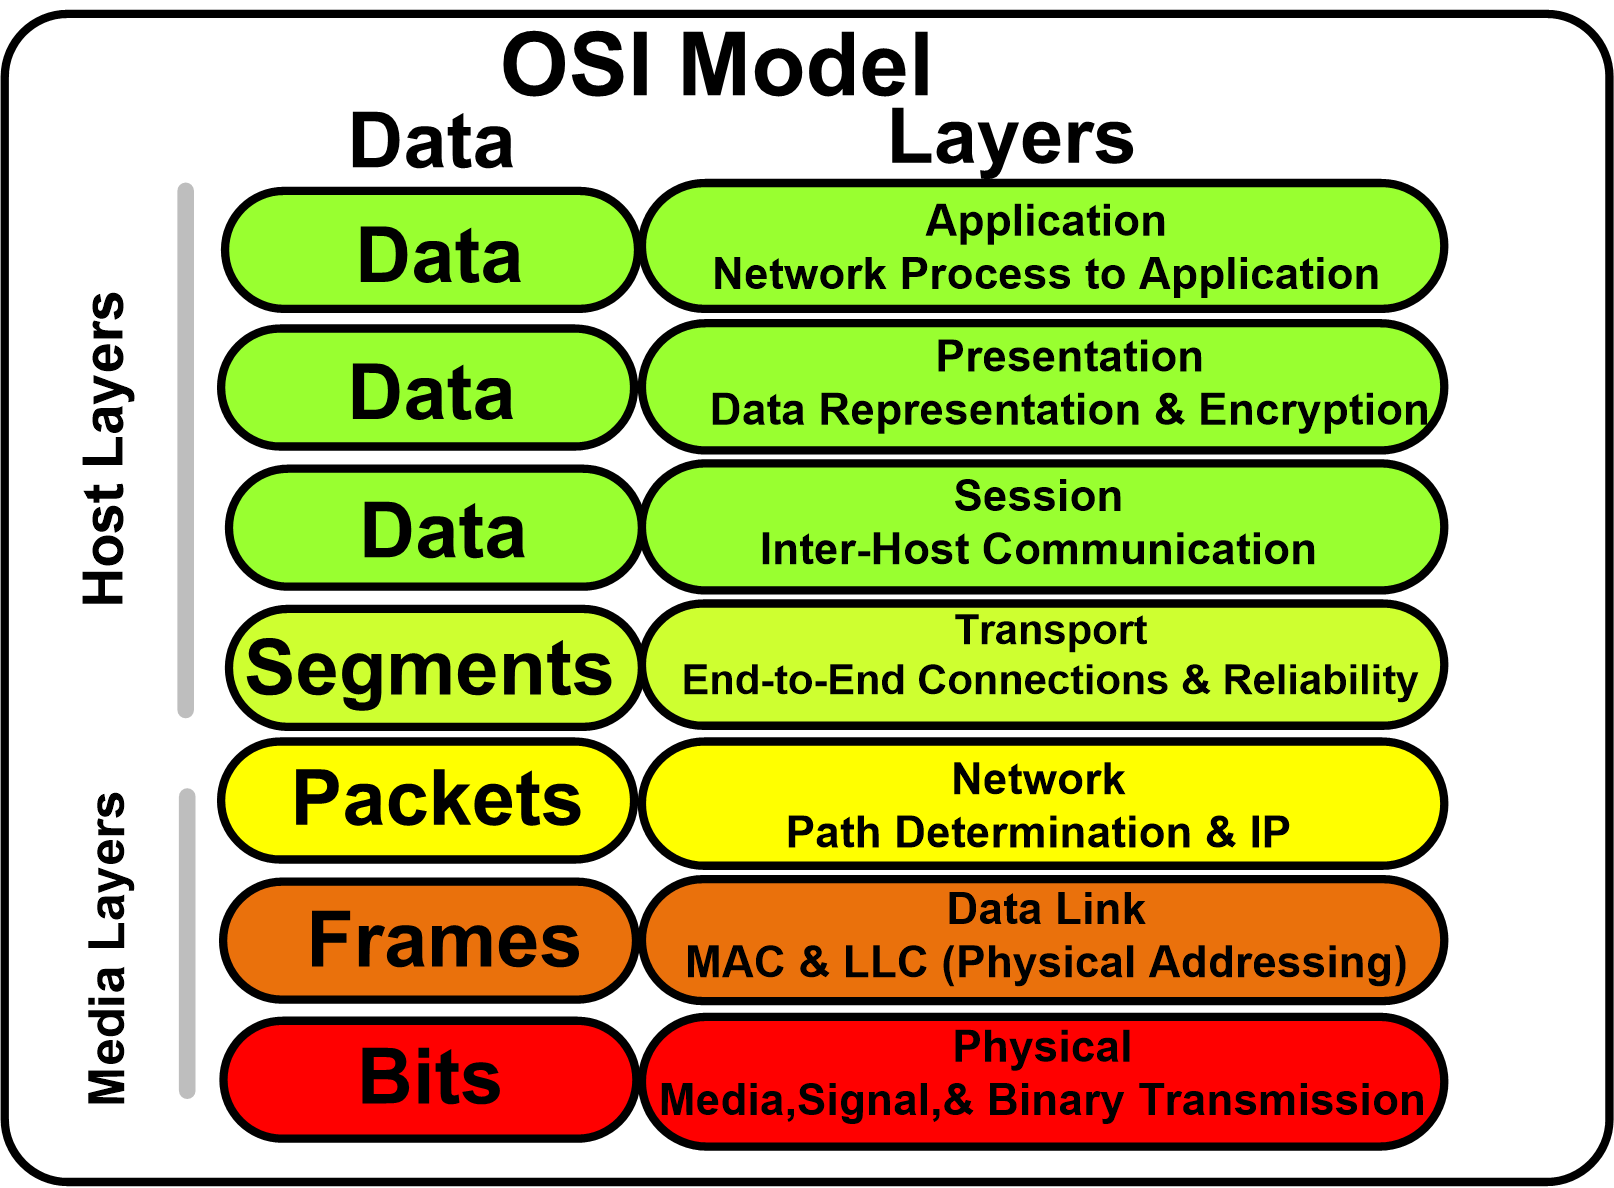
\includegraphics[scale=0.125]{osi}
           \end{tabular}
\end{tabular}\\
\end{tabular}
\end{frame}

\section{Network Layer}
\subsection{Aufgaben}
\begin{frame}
	\frametitle{Network Layer}
	\begin{itemize}
		\item Weiterleitung von Paketen über Zwischenrechner zum Ziel (Forwarding)
		\item Wahl der Routen, Anpassung, Optimierung (Routing)
		\item Vermittlungsarten: Leitungsvermittlung vs. Paketvermittlung
		\item Für die Übungen (Routing): Paketvermittlung
	\end{itemize}
\end{frame}

\subsection{Geräte -- Router \& Gateways}
\begin{frame}
	\frametitle{Geräte -- Router}
	\vspace{-0.75cm}
	\begin{itemize}
		\item Router
		\begin{itemize}
			\item Verbindet logische Netze miteinander; leitet Datenpakete weiter (Zwischenknoten)
			\item Hat gültige Adresse in jedem angeschlossenen Netz
			\item Kennt i.d.R. Wege zu anderen Netzwerken!
			\item Besitzt i.d.R. mehrere Schnittstellen (wie Hub \& Switch)
			\begin{itemize}
				\item Raspberry Pi hat nur ein echten physikalischen Ethernet-Adapter
				\item Keine Sorge, wir basteln uns mehrere virtuelle Adapter
			\end{itemize}
		\end{itemize}				
	\end{itemize}
\end{frame}
\begin{frame}
	\frametitle{Geräte -- Gateways}
	\begin{itemize}
		\item Gateway
		\begin{itemize}
			\item Ermöglicht Kommunikation zwischen Netzen mit unterschiedlichen Protokollen -- Protokollübersetzung
			\item Kann theoretisch auf allen Schichten des OSI-Modells arbeiten
			\item Gateways die auf Vermittlungsschicht-Ebene arbeiten, heißen auch Mehrprotokoll-/ Multiprotokoll-Router
		\end{itemize}
		\item Access-Gateway (Dial-In Router)
		\begin{itemize}
			\item Ermöglicht Verbindung eines Ethernet-Netzwerks (LAN) mit einem WAN (z.B. via DSL, 3G/4G Mobilfunk)
		\end{itemize}
	\end{itemize}
\end{frame}

\subsection{Adressierung}
\begin{frame}
	\frametitle{Adressierung}
	\vspace{-0.75cm}
	\begin{itemize}
		\item Schicht 2: Physische Adressen
		\begin{itemize}
			\item Nachrichtenversand durch Ansprechen tatsächlicher, physischer Geräte
			\item Weiterleitung vorwiegend elektrisch (Repeater, Hubs) bzw. mit minimaler Fehlerprüfung (Switches)
		\end{itemize}
		\item Schicht 3: Logische Adressen
		\begin{itemize}
			\item Entkopplung tatsächlich, physischer Ebene von semantisch, logischer Ebene
			\item Hierarchiebildung auf logischer Ebene (Netzbildung)
			\item Wegwahl \& Weiterleitung (Forwarding \& Routing) auf Basis logischer Adressen
			\item Kommunikation über verschiedene Netze/Broadcast-Domänen hinweg
			\item Nachrichten müssen von Gerät zu Gerät transportiert werden $\rightarrow$ Nachricht muss
bei jeder Weiterleitung neu adressiert werden
			\item Logische Adressen als zweites Adressierungsschema zur Beibehaltung von Ende-zu-Ende Adressen
		\end{itemize}
	\end{itemize}
\end{frame}

\section{Tools}
\begin{frame}
	\frametitle{Tools}
	\vspace{-0.75cm}
	\url{http://xmodulo.com/linux-tcpip-networking-net-tools-iproute2.html}
	\begin{itemize}
		\item \emph{iproute2}
		\begin{itemize}
			\item ip addr -- Netzwerkinterface + Adresse
			\item ip link -- nur Interface
			\item ip route -- Routing Informationen \& Routing-Tabelle
			\item ip route [add|delete|...] \emph{net\_addr} via \emph{gateway} dev \emph{device\_name}
		\end{itemize}
		\item \emph{net-tools}
		\begin{itemize}
			\item ifconfig -- Netzwerkinterface + Adresse
			\item route -n -- Routen anzeigen
			\item netstat -rn
			\item route add -net \emph{net\_addr} gw \emph{gateway} dev \emph{device\_name}
			\item route del -net \emph{net\_addr}
		\end{itemize}
	\end{itemize}
\end{frame}

\begin{frame}
	\frametitle{Tools II -- OS}
	\begin{itemize}
		\item Routing ist deutlich komplexer $\rightarrow$ Aufgabe des Betriebssystems bzw. der Hard- \& Software des Routers
		\item BS sorgt für das Finden von Routen und das weiterleiten von Paketen
		\item Routing erfolgt aufgrund von Routing-Algorithmen (Dijkstra- \& Bellman-Ford-Algorithmus)
		\item Routing muss explizit erlaubt werden!
	\end{itemize}
\end{frame}

\section{Empfehlungen}
\begin{frame}{Nerd-Wochenmarkt}
Empfehlung der Woche:
\begin{itemize}
	\item Request for Comments -- Der RFC Podcast
	\begin{itemize}
		\item IP Routing I: \url{https://requestforcomments.de/archives/343}
		\item IP Routing II: \url{https://requestforcomments.de/archives/351}
		\item IP Routing III: \url{https://requestforcomments.de/archives/374}   
	\end{itemize}
	\item Datengarten des CCCB
	\begin{itemize}
		\item Technik und Wahrheit \url{https://media.ccc.de/v/dg-82}
	\end{itemize}
\end{itemize}
\end{frame}

\end{document}